% Chapter X

\chapter{Estensione del metodo alle linee ferroviarie} % Chapter title
A partire dal metodo precendentemente descritto per gli edifici si è pensato di estendere il medesimo criterio anche alle rotte. Per rotta si intende una tratta che può essere una semplice strada, autostrata, o anche una linea ferroviaria sul quale bisogna effettuare lo studio di rischio frana alla quale potrebbe essere soggetta. Il metodo di base sviluppato per gli edifici calcolava il valore di exposure di determinati asset che erano riducibili a semplici punti geografici. Si deduce pertanto che l'estensione di tale metodo alle rotte richiede il campionamento di queste per approssimarle ad una serie di punti.
Prima di proseguire nel metodo bisogna definire alcune notazioni:

\begin{enumerate}
	\setcounter{enumi}{18}
	\item \textbf{$ \mathcal{R} $ (Routes)} $ = \{r_k(k=1,..,\mathbf{card}(\mathcal{R}) | r_k $ è una \textit{Route} ubicata all'interno dei confini della  GeoArea \}. Per \textit{Route} si intende una generica tratta (come ad esempio una ferrovia, un'autostrada) descritta dalla tupla < \textit{ID}, \textit{Name}, \textit{geometry}>. Il campo \textit{ID} identifica univocamente la tratta; \textit{Name} una sua etichetta nominale; \textit{geometry} rappresenta una geometria che descrive la tratta sul territorio. Nelle notazioni introdotte di seguito l'occorrenza del pedice $\{k\}$ viene usata $sempre$ per richiamare la \textit{Route} $k-esima$, ovvero alla tratta $r_k$ di $ \mathcal{R} $.
	
		\begin{figure}[h]
		\centering
		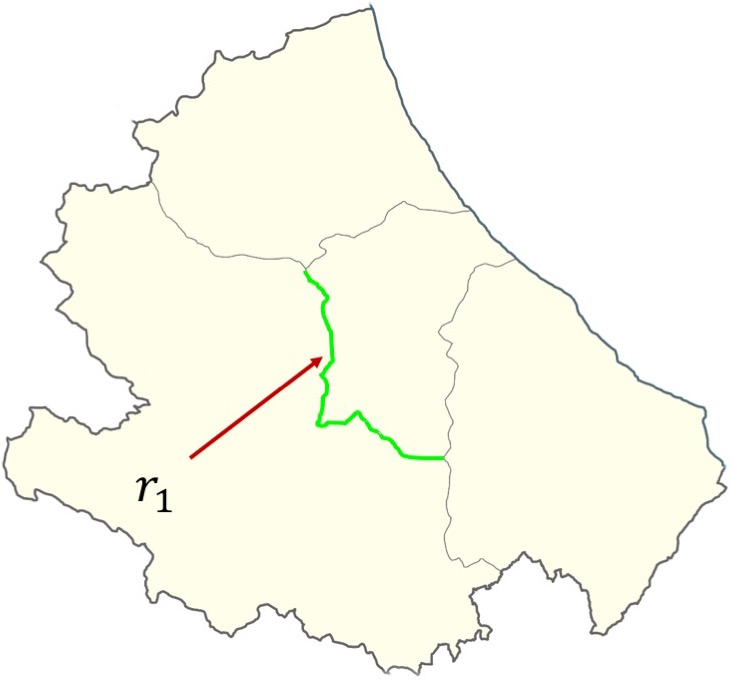
\includegraphics[width=0.4\textwidth]{images/routes1}
		\caption{la linea verde rappresenta la \textit{Route} $r_1$ dell'insieme $ \mathcal{R} $}
		\label{img:route}
		\end{figure}
	
	\item \textbf{$ \mathcal{RS}_k $ (Route Segments)} $ = \{rs_{k,s}(k=1,..,\mathbf{card}(\mathcal{R})),(s=1,..,\mathbf{card}(\mathcal{RS}_k))  | rs_{k,s} $ è una \textit{Route Segment} di una specifica \textit{Route} $r_k$ \}. Per \textit{Route Segment} $rs_{k,s}$ si intende la sotto-tratta $s-esima$ di lunghezza $v$ della \textit{Route} $r_k$. L'unione di tutti gli $rs_{k,s}$ restituisce l'elemento $r_k$. Nelle notazioni introdotte di seguito l'occorrenza del pedice $\{k,s\}$ viene usata $sempre$ per richiamare che ci si riferisce al \textit{Route Segment} $s-esimo$ della \textit{Route} $k-esima$.
		
	\item \textbf{$ \mathcal{RSP}_{k,s} $ (Route Segment Points)} $ = \{rsp_{k,s,p}(k=1,..,\mathbf{card}(\mathcal{R})),(s=1,..,\mathbf{card}(\mathcal{RS}_k)),(p=1,..,\mathbf{card}(\mathcal{RSP}_{k,s}))  | rsp_{k,s,p} $ è una \textit{Route Segment Point} di una specifica \textit{Route Segment} \}. Per \textit{Route Segment Point} $rsp_{k,s,p}$ si intende il $p-esimo$ punto ottenuto dal campionamento della \textit{Route Segment} $rs_{k,s}$. L'insieme di tutti gli $rsp_{k,s,p}$ con $k$ ed $s$ fissati, equivalgono all'inisieme di tutti i punti risultanti dal campionamento di $rs_{k,s}$.
	
\end{enumerate}

\noindent Il metodo consiste nel calcolare i valori di exposure delle \textit{Route Segments} di ogni \textit{Route} interna alla \textit{GeoArea}.
Il primo passo consiste nel "Segmentare" ogni tratta $r_k$ in sotto-tratte di lunghezza $v$ in modo da ottenerne:

\begin{equation}\label{eq:numerotratte}
m_{k}=\left\lceil\left(\frac{Lunghezza(r_k)}{v}\right)\right\rceil
\end{equation}
\\
Il numero $m_{k}$ di sotto-tratte è pari all'arrotondamento in eccesso tra il rapporto della lunghezza della tratta $r_k$ e il passo di segmentazione $v$. Si può intuire che tutte le sotto-tratte avranno lunghezza pari a $v$ eccetto l'ultima che avrà una lunghezza minore o al massimo uguale. Il valore di $m_k$ corrisponde pertanto alla $\mathbf{card}(\mathcal{RS}_{k})$
\\


	\begin{figure}[h]
	\centering
	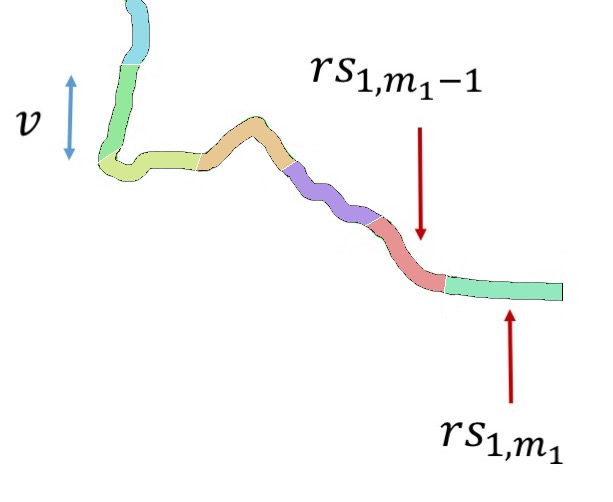
\includegraphics[width=0.4\textwidth]{images/routes2_new}
	\caption{Nella figura viene mostrata la procedura di segmentazione di una \textit{Route} in sotto-tratte di lunghezza $v$. Si può notare in questo caso che  l'ultima sotto-tratta $rs_{1,{m_1}}$ ha lunghezza inferiore a $v$}
	\label{img:segment}
	\end{figure}

\noindent A questo punto, ogni sotto-tratta $rs_{k,s}$ dovrà essere campionata ed approssimata ad una serie di punti. Si definisce pertanto un passo di campionamento $q << v$ che rappresenta la distanza massima tra i punti. Il numero di punti risultanti dal campionamento della sotto-tratta $rs_{k,s}$ sarà:

\begin{equation}\label{eq:numerotratte}
n_{k,s}=\left\lceil\left(\frac{Lunghezza(rs_{k,s})}{q}\right)\right\rceil
\end{equation}
\\
Al termine del campionamento, tutti i punti avranno una distanza dagli adiacenti pari al passo di campionamento ad eccezione dell'ultimo che avrà una distanza $\le q$ (Figura \ref{img:campionamento} e \ref{img:campionamento_2}). Pertanto si consiglia un passo di campionamento $q$ che sia divisibile per $v$ (in questo modo l'unico punto ad avere distanza $\le q$ dai vicini sarà l'ultimo punto della ultima sotto-tratta di $r_k$ ) Il valore di $n_{k,s}$ corrisponde alla $\mathbf{card}(\mathcal{RSP}_{k,s})$
\\

\begin{figure}[h]
	\centering
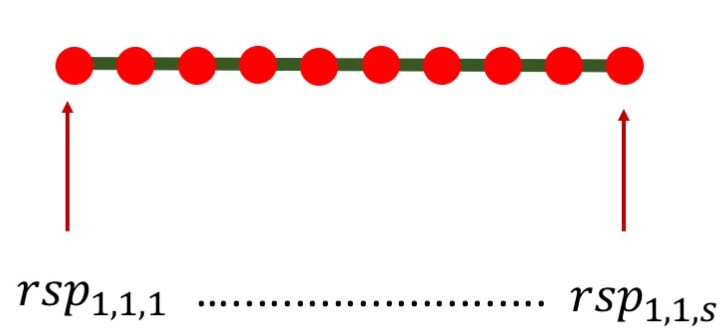
\includegraphics[width=0.6\textwidth]{images/routes3}
\caption{Esempio di campionamento di una \textit{Route Segment} con passo di campionamento $q$ (Caso con $v$ divisibile per $q$) }
\label{img:campionamento}
\end{figure}

\begin{figure}[h]
	\centering
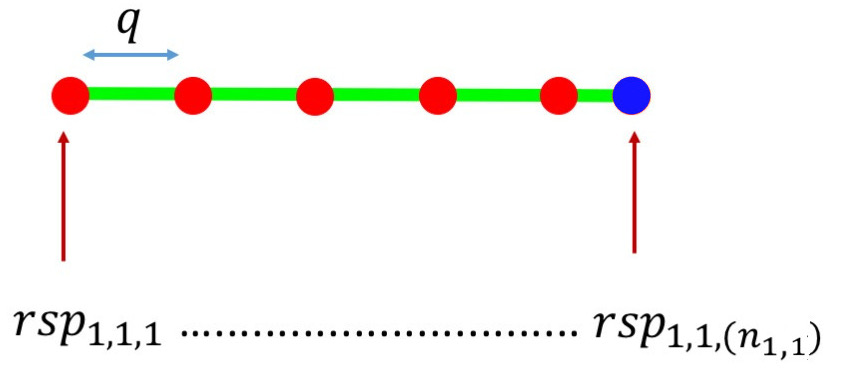
\includegraphics[width=0.6\textwidth]{images/routes4}
\caption{Esempio di campionamento di una \textit{Route Segment} con passo di campionamento $q$ (Caso con $v$ non divisibile per $q$). Si nota in questo caso l'ultimo punto di colore blue si trova a distanza <$q$ dall'adiacente }
\label{img:campionamento_2}
\end{figure}

\newpage
\noindent Una volta ottenuti i punti $rsp_{k,s,p}$ che approssimano la sotto-tratta $rs_{k,s}$, è possibile applicare il metodo base di calcolo per l'exposure. Per il metodo esteso alle tratte, si è deciso di lavorare su due sistemi diversi per la rappresentazione della exposure. Le definiamo con le seguenti notazioni:

\begin{enumerate}
\setcounter{enumi}{21}
\item \label{ERSP} \textbf{$ExpRSP$ (Exposure Route Segment Points)} =\\
$ \{exprsp_{k,s,p} (k=1,..,\mathbf{card}(\mathcal{R})),(s=1,..,\mathbf{card}(\mathcal{RS}_k)),(p=1,..,\mathbf{card}(\mathcal{RSP}_{k,s}))  | exprsp_{k,s,p} $ è il valore di \textit{exposure} del $p-esimo$ punto della sotto-tratta $rs_{k,s}$. Esso è descritto dalla tupla \textit{<ID,name,km,position,exposure>} ove \textit{ID} identifica univocamente il punto; \textit{name} rappresenta il nome della $r_k$ di appartenenza; \textit{km} identifica a quale sotto-tratta di $r_k$ ci si riferisce; \textit{position} rappresenta la posizione geografica di $rsp_{k,s,p}$; \textit{exposure} indica il valore di exposure del relativo punto.

\item \label{ERS} \textbf{$ExpRS$ (Exposure Route Segment)} =\\$ \{Exprs_{k,s} (k=1,..,\mathbf{card}(\mathcal{R})),(s=1,..,\mathbf{card}(\mathcal{RS}_k)) | exprs_{k,s} $ è il valore di \textit{exposure} della sotto-tratta $s-esima$ della tratta $r_k$. Esso è descritto dalla tupla \textit{<km,name,geometry,exposure>} ove \textit{km} identifica a quale sotto-tratta di $r_k$ ci si riferisce; \textit{name} rappresenta il nome della $r_k$ di appartenenza; \textit{geometry} rappresenta la geometria di $rs_{k,s}$, \textit{exposure} indica il valore di exposure della relativa sotto-tratta, intesa come sommatoria delle exposure dei punti $rsp_{k,s,p}$ della medesima. Ogni tupla è univocamente identificabile dalla coppia [km,name].

\end{enumerate}
\noindent Il primo sistema, rappresenta l'exposure per i singoli punti $rsp_{k,s,p}$ trattandoli come se fossero edifici $b_i$. Pertanto si applica lo stesso metodo del \textit{Capitolo 3} così da cacolare i valori di exposure per ogni punto. Infine tale risultato sarà rappresentato secondo la notazione \ref{ERSP}.
\bigbreak
\noindent Il secondo sistema invece parte dai risultati ottenuti dal primo ma ha l'obettivo di rappresentare l'exposure non per i singoli punti ma per le specifiche sotto-tratte $rs_{k,s}$. Il valore di exposure per singola sotto-tratta è data dalla seguente equazione:

\begin{equation}\label{eq:exprs}
exprs_{k,s}=\frac{1}{n_{k,s}}\left(\sum_{p=1}^{n_{k,s}} exprsp_{k,s,p}\right)
\end{equation}


\noindent Con parole esplicite, l'exposure di una sotto-tratta $rs_{k,s}$ equivale alla media delle exposure di tutti i punti $rsp_{k,s,p}$ ottenuti dal suo campionamento. Il risultato sarà rappresentato secondo la notazione \ref{ERS}.

\section{Validazione del metodo}
Le rotte della regione Abruzzo sono le seguenti:
\begin{enumerate}
	\item Bologna - Bari
	\item Roma - Pescara
	\item Ortona - Crocetta
	\item Marina di San Vito - Castel di Sangro
	\item Teramo - Giulianova
	\item Avezzano - Roccasecca
	\item Sulmona - Carpinone
	\item Rieti - L'Aquila - Sulmona
	\item Archi stazione - Atessa
\end{enumerate}
Ciascuna di esse è stata suddivisa in sotto-tratte di 1500 metri, campionata successivamente con un passo di 300 metri. 
I risultati dell'exposure sulle sotto-tratte sono riportati nella tabella \ref{tabella-risultati-rotte}. La colorazione delle classi di appartenenza è la stessa di quella vista per le stazioni (rosso classe alta, giallo classe media e verde classe bassa).

\subsection{Bologna - Bari}

\tiny
% Please add the following required packages to your document preamble:
% \usepackage[table,xcdraw]{xcolor}
% If you use beamer only pass "xcolor=table" option, i.e. \documentclass[xcolor=table]{beamer}
\begin{table}[H]
	\centering
	\caption{My caption}
	\label{my-label}
	\begin{tabular}{|
			>{\columncolor[HTML]{32CB00}}l |
			>{\columncolor[HTML]{32CB00}}l |l|
			>{\columncolor[HTML]{32CB00}}l |
			>{\columncolor[HTML]{32CB00}}l |lll}
		\cline{1-2} \cline{4-5} \cline{7-8}
		\multicolumn{1}{|c|}{\cellcolor[HTML]{C0C0C0}\textbf{Km}} & \multicolumn{1}{c|}{\cellcolor[HTML]{C0C0C0}\textbf{Exposure}} & \multicolumn{1}{c|}{\textbf{}} & \multicolumn{1}{c|}{\cellcolor[HTML]{C0C0C0}\textbf{Km}} & \multicolumn{1}{c|}{\cellcolor[HTML]{C0C0C0}\textbf{Exposure}} & \multicolumn{1}{c|}{\textbf{}}               & \multicolumn{1}{c|}{\cellcolor[HTML]{C0C0C0}\textbf{Km}} & \multicolumn{1}{c|}{\cellcolor[HTML]{C0C0C0}\textbf{Exposure}} \\ \cline{1-2} \cline{4-5} \cline{7-8} 
		\cellcolor[HTML]{F8FF00}40.5                              & \cellcolor[HTML]{F8FF00}0.340594968                            &                                & 78                                                       & 0.108499965                                                    & \multicolumn{1}{l|}{{\color[HTML]{000000} }} & \multicolumn{1}{l|}{\cellcolor[HTML]{32CB00}9}           & \multicolumn{1}{l|}{\cellcolor[HTML]{32CB00}0.005637561}       \\ \cline{1-2} \cline{4-5} \cline{7-8} 
		\cellcolor[HTML]{F8FF00}39                                & \cellcolor[HTML]{F8FF00}0.311711099                            &                                & 87                                                       & 0.107982258                                                    & \multicolumn{1}{l|}{}                        & \multicolumn{1}{l|}{\cellcolor[HTML]{32CB00}109.5}       & \multicolumn{1}{l|}{\cellcolor[HTML]{32CB00}0.005057386}       \\ \cline{1-2} \cline{4-5} \cline{7-8} 
		\cellcolor[HTML]{F8FF00}49.5                              & \cellcolor[HTML]{F8FF00}0.307784618                            &                                & 57                                                       & 0.103736722                                                    & \multicolumn{1}{l|}{}                        & \multicolumn{1}{l|}{\cellcolor[HTML]{32CB00}54}          & \multicolumn{1}{l|}{\cellcolor[HTML]{32CB00}0.003521025}       \\ \cline{1-2} \cline{4-5} \cline{7-8} 
		\cellcolor[HTML]{F8FF00}94.5                              & \cellcolor[HTML]{F8FF00}0.245124558                            &                                & 67.5                                                     & 0.102103561                                                    & \multicolumn{1}{l|}{}                        & \multicolumn{1}{l|}{\cellcolor[HTML]{32CB00}106.5}       & \multicolumn{1}{l|}{\cellcolor[HTML]{32CB00}0.002007457}       \\ \cline{1-2} \cline{4-5} \cline{7-8} 
		\cellcolor[HTML]{F8FF00}76.5                              & \cellcolor[HTML]{F8FF00}0.237416449                            &                                & 36                                                       & 0.096267953                                                    & \multicolumn{1}{l|}{}                        & \multicolumn{1}{l|}{\cellcolor[HTML]{32CB00}12}          & \multicolumn{1}{l|}{\cellcolor[HTML]{32CB00}0}                 \\ \cline{1-2} \cline{4-5} \cline{7-8} 
		\cellcolor[HTML]{F8FF00}63                                & \cellcolor[HTML]{F8FF00}0.236921131                            &                                & 7.5                                                      & 0.095320484                                                    & \multicolumn{1}{l|}{}                        & \multicolumn{1}{l|}{\cellcolor[HTML]{32CB00}18}          & \multicolumn{1}{l|}{\cellcolor[HTML]{32CB00}0}                 \\ \cline{1-2} \cline{4-5} \cline{7-8} 
		\cellcolor[HTML]{F8FF00}75                                & \cellcolor[HTML]{F8FF00}0.230552616                            &                                & 61.5                                                     & 0.091809053                                                    & \multicolumn{1}{l|}{}                        & \multicolumn{1}{l|}{\cellcolor[HTML]{32CB00}28.5}        & \multicolumn{1}{l|}{\cellcolor[HTML]{32CB00}0}                 \\ \cline{1-2} \cline{4-5} \cline{7-8} 
		\cellcolor[HTML]{F8FF00}81                                & \cellcolor[HTML]{F8FF00}0.229742314                            &                                & 70.5                                                     & 0.090962663                                                    & \multicolumn{1}{l|}{}                        & \multicolumn{1}{l|}{\cellcolor[HTML]{32CB00}45}          & \multicolumn{1}{l|}{\cellcolor[HTML]{32CB00}0}                 \\ \cline{1-2} \cline{4-5} \cline{7-8} 
		\cellcolor[HTML]{F8FF00}51                                & \cellcolor[HTML]{F8FF00}0.225002677                            &                                & 97.5                                                     & 0.08941622                                                     & \multicolumn{1}{l|}{}                        & \multicolumn{1}{l|}{\cellcolor[HTML]{32CB00}46.5}        & \multicolumn{1}{l|}{\cellcolor[HTML]{32CB00}0}                 \\ \cline{1-2} \cline{4-5} \cline{7-8} 
		82.5                                                      & 0.191829629                                                    &                                & 52.5                                                     & 0.085691274                                                    & \multicolumn{1}{l|}{}                        & \multicolumn{1}{l|}{\cellcolor[HTML]{32CB00}66}          & \multicolumn{1}{l|}{\cellcolor[HTML]{32CB00}0}                 \\ \cline{1-2} \cline{4-5} \cline{7-8} 
		114                                                       & 0.190609033                                                    &                                & 105                                                      & 0.08198181                                                     & \multicolumn{1}{l|}{}                        & \multicolumn{1}{l|}{\cellcolor[HTML]{32CB00}111}         & \multicolumn{1}{l|}{\cellcolor[HTML]{32CB00}0}                 \\ \cline{1-2} \cline{4-5} \cline{7-8} 
		3                                                         & 0.189954036                                                    &                                & 72                                                       & 0.079795991                                                    & \multicolumn{1}{l|}{}                        & \multicolumn{1}{l|}{\cellcolor[HTML]{32CB00}121.5}       & \multicolumn{1}{l|}{\cellcolor[HTML]{32CB00}0}                 \\ \cline{1-2} \cline{4-5} \cline{7-8} 
		115.5                                                     & 0.17680531                                                     &                                & 58.5                                                     & 0.072116987                                                    & \multicolumn{1}{l|}{}                        & \multicolumn{1}{l|}{\cellcolor[HTML]{32CB00}123}         & \multicolumn{1}{l|}{\cellcolor[HTML]{32CB00}0}                 \\ \cline{1-2} \cline{4-5} \cline{7-8} 
		117                                                       & 0.176498763                                                    &                                & 4.5                                                      & 0.066458812                                                    &                                              &                                                          &                                                                \\ \cline{1-2} \cline{4-5}
		33                                                        & 0.168217446                                                    &                                & 1.5                                                      & 0.063656129                                                    &                                              &                                                          &                                                                \\ \cline{1-2} \cline{4-5}
		96                                                        & 0.163999295                                                    &                                & 103.5                                                    & 0.063337462                                                    &                                              &                                                          &                                                                \\ \cline{1-2} \cline{4-5}
		0                                                         & 0.160867925                                                    &                                & 64.5                                                     & 0.061186773                                                    &                                              &                                                          &                                                                \\ \cline{1-2} \cline{4-5}
		15                                                        & 0.158064282                                                    &                                & 34.5                                                     & 0.054063351                                                    &                                              &                                                          &                                                                \\ \cline{1-2} \cline{4-5}
		85.5                                                      & 0.157229062                                                    &                                & 112.5                                                    & 0.052424689                                                    &                                              &                                                          &                                                                \\ \cline{1-2} \cline{4-5}
		22.5                                                      & 0.152140373                                                    &                                & 25.5                                                     & 0.0503954                                                      &                                              &                                                          &                                                                \\ \cline{1-2} \cline{4-5}
		31.5                                                      & 0.14457745                                                     &                                & 16.5                                                     & 0.04617001                                                     &                                              &                                                          &                                                                \\ \cline{1-2} \cline{4-5}
		118.5                                                     & 0.142523857                                                    &                                & 93                                                       & 0.041641969                                                    &                                              &                                                          &                                                                \\ \cline{1-2} \cline{4-5}
		24                                                        & 0.142488217                                                    &                                & 102                                                      & 0.039718736                                                    &                                              &                                                          &                                                                \\ \cline{1-2} \cline{4-5}
		37.5                                                      & 0.141178199                                                    &                                & 99                                                       & 0.028661674                                                    &                                              &                                                          &                                                                \\ \cline{1-2} \cline{4-5}
		69                                                        & 0.140380246                                                    &                                & 6                                                        & 0.026834452                                                    &                                              &                                                          &                                                                \\ \cline{1-2} \cline{4-5}
		13.5                                                      & 0.1352954                                                      &                                & 91.5                                                     & 0.02612962                                                     &                                              &                                                          &                                                                \\ \cline{1-2} \cline{4-5}
		42                                                        & 0.132707801                                                    &                                & 19.5                                                     & 0.024434587                                                    &                                              &                                                          &                                                                \\ \cline{1-2} \cline{4-5}
		21                                                        & 0.130976328                                                    &                                & 10.5                                                     & 0.022974444                                                    &                                              &                                                          &                                                                \\ \cline{1-2} \cline{4-5}
		60                                                        & 0.130473609                                                    &                                & 120                                                      & 0.022885286                                                    &                                              &                                                          &                                                                \\ \cline{1-2} \cline{4-5}
		48                                                        & 0.130252994                                                    &                                & 43.5                                                     & 0.022815119                                                    &                                              &                                                          &                                                                \\ \cline{1-2} \cline{4-5}
		84                                                        & 0.127211536                                                    &                                & 55.5                                                     & 0.018851821                                                    &                                              &                                                          &                                                                \\ \cline{1-2} \cline{4-5}
		90                                                        & 0.124353161                                                    &                                & 27                                                       & 0.018389377                                                    &                                              &                                                          &                                                                \\ \cline{1-2} \cline{4-5}
		73.5                                                      & 0.12079172                                                     &                                & 100.5                                                    & 0.015003722                                                    &                                              &                                                          &                                                                \\ \cline{1-2} \cline{4-5}
		88.5                                                      & 0.116672291                                                    &                                & 30                                                       & 0.009969652                                                    &                                              &                                                          &                                                                \\ \cline{1-2} \cline{4-5}
		79.5                                                      & 0.108806841                                                    &                                & 108                                                      & 0.007064843                                                    &                                              &                                                          &                                                                \\ \cline{1-2} \cline{4-5}
	\end{tabular}
\end{table}

\normalsize

\begin{table}[H]
	\centering
	\caption{My caption}
	\label{risultati_bologna_bari}
	\begin{tabular}{|c|c|c|}
		\hline
		\rowcolor[HTML]{C0C0C0} 
		\textbf{Exposure} & \textbf{\# hotspot} & \textbf{\% di hotspot per exposure} \\ \hline
		Classe Alta       & 0                   & 0                                   \\ \hline
		Classe Media      & 9                  & 10.84                               \\ \hline
		Classe Bassa      & 74                 & 89.16                               \\ \hline
		Tot. Hotspot      & 83                 & 100                                 \\ \hline
	\end{tabular}
\end{table}



\subsection{Roma - Pescara}

\begin{longtable}{|l|l|}
	\centering
	\rowcolor[HTML]{9B9B9B} \textbf{Km} & \textbf{Exposure} \\ \hline
	\rowcolor[HTML]{FE0000} 45                                                      & 1.966849682                                                   \\
 \rowcolor[HTML]{FE0000} 
 156                                                     & 1.394371844                                                   \\
 \rowcolor[HTML]{FE0000} 
 46.5                                                    & 1.384893057                                                   \\
 \rowcolor[HTML]{FE0000} 
 85.5                                                    & 1.346763995                                                   \\
 \rowcolor[HTML]{FE0000} 
 96                                                      & 1.303709059                                                   \\
 \rowcolor[HTML]{FE0000} 
 87                                                      & 1.279284765                                                   \\
 \rowcolor[HTML]{FE0000} 
 76.5                                                    & 1.257479083                                                   \\
 \rowcolor[HTML]{FE0000} 
 75                                                      & 1.243870549                                                   \\
 \rowcolor[HTML]{FE0000} 
 48                                                      & 1.241289783                                                   \\
 \rowcolor[HTML]{FE0000} 
 84                                                      & 1.217226497                                                   \\
 \rowcolor[HTML]{FE0000} 
 94.5                                                    & 1.214614543                                                   \\
 \rowcolor[HTML]{FE0000} 
 43.5                                                    & 1.159685769                                                   \\
 \rowcolor[HTML]{FE0000} 
 157.5                                                   & 1.132398042                                                   \\
 \rowcolor[HTML]{FE0000} 
 154.5                                                   & 1.109263462                                                   \\
 \rowcolor[HTML]{F8FF00} 
 88.5                                                    & 1.073736159                                                   \\
 \rowcolor[HTML]{F8FF00} 
 99                                                      & 1.071011754                                                   \\
 \rowcolor[HTML]{F8FF00} 
 82.5                                                    & 1.0432196                                                     \\
 \rowcolor[HTML]{F8FF00} 
 153                                                     & 1.033151328                                                   \\
 \rowcolor[HTML]{F8FF00} 
 49.5                                                    & 1.019767856                                                   \\
 \rowcolor[HTML]{F8FF00} 
 97.5                                                    & 1.003135081                                                   \\
 \rowcolor[HTML]{F8FF00} 
 78                                                      & 0.853151579                                                   \\
 \rowcolor[HTML]{F8FF00} 
 105                                                     & 0.845812478                                                   \\
 \rowcolor[HTML]{F8FF00} 
 81                                                      & 0.835046678                                                   \\
 \rowcolor[HTML]{F8FF00} 
 93                                                      & 0.831040595                                                   \\
 \rowcolor[HTML]{F8FF00} 
 79.5                                                    & 0.777983975                                                   \\
 \rowcolor[HTML]{F8FF00} 
 103.5                                                   & 0.761000733                                                   \\
 \rowcolor[HTML]{F8FF00} 
 73.5                                                    & 0.7303475                                                     \\
 \rowcolor[HTML]{F8FF00} 
 126                                                     & 0.730055945                                                   \\
 \rowcolor[HTML]{F8FF00} 
 162                                                     & 0.681525635                                                   \\
 \rowcolor[HTML]{F8FF00} 
 90                                                      & 0.640480046                                                   \\
 \rowcolor[HTML]{F8FF00} 
 100.5                                                   & 0.623288543                                                   \\
 \rowcolor[HTML]{F8FF00} 
 147                                                     & 0.592425294                                                   \\
 \rowcolor[HTML]{F8FF00} 
 118.5                                                   & 0.587927716                                                   \\
 \rowcolor[HTML]{F8FF00} 
 124.5                                                   & 0.580918957                                                   \\
 \rowcolor[HTML]{F8FF00} 
 148.5                                                   & 0.578028267                                                   \\
 \rowcolor[HTML]{F8FF00} 
 102                                                     & 0.560250703                                                   \\
 \rowcolor[HTML]{F8FF00} 
 160.5                                                   & 0.55711672                                                    \\
 \rowcolor[HTML]{F8FF00} 
 42                                                      & 0.555368862                                                   \\
 \rowcolor[HTML]{F8FF00} 
 117                                                     & 0.523293613                                                   \\
 \rowcolor[HTML]{F8FF00} 
 163.5                                                   & 0.521084606                                                   \\
 \rowcolor[HTML]{F8FF00} 
 159                                                     & 0.516866205                                                   \\
 \rowcolor[HTML]{F8FF00} 
 151.5                                                   & 0.512931338                                                   \\
 \rowcolor[HTML]{F8FF00} 
 40.5                                                    & 0.471466063                                                   \\
 \rowcolor[HTML]{F8FF00} 
 150                                                     & 0.465822645                                                   \\
 \rowcolor[HTML]{F8FF00} 
 91.5                                                    & 0.465646587                                                   \\
 \rowcolor[HTML]{F8FF00} 
 39                                                      & 0.461957679                                                   \\
 \rowcolor[HTML]{F8FF00} 
 135                                                     & 0.414594346                                                   \\
 \rowcolor[HTML]{F8FF00} 
 115.5                                                   & 0.405512318                                                   \\
 \rowcolor[HTML]{F8FF00} 
 106.5                                                   & 0.373471504                                                   \\
 \rowcolor[HTML]{F8FF00} 
 37.5                                                    & 0.370922337                                                   \\
 \rowcolor[HTML]{F8FF00} 
 30                                                      & 0.35504666                                                    \\
 \rowcolor[HTML]{F8FF00} 
 109.5                                                   & 0.346937564                                                   \\
 \rowcolor[HTML]{F8FF00} 
 51                                                      & 0.341668219                                                   \\
 \rowcolor[HTML]{F8FF00} 
 36                                                      & 0.339037556                                                   \\
 \rowcolor[HTML]{F8FF00} 
 133.5                                                   & 0.337786441                                                   \\
 \rowcolor[HTML]{F8FF00} 
 108                                                     & 0.334736603                                                   \\
 \rowcolor[HTML]{F8FF00} 
 31.5                                                    & 0.333363304                                                   \\
 \rowcolor[HTML]{F8FF00} 
 33                                                      & 0.332700364                                                   \\
 \rowcolor[HTML]{F8FF00} 
 111                                                     & 0.31580843                                                    \\
 \rowcolor[HTML]{F8FF00} 
 145.5                                                   & 0.309075866                                                   \\
 \rowcolor[HTML]{F8FF00} 
 120                                                     & 0.266754253                                                   \\
 \rowcolor[HTML]{F8FF00} 
 72                                                      & 0.265690267                                                   \\
 \rowcolor[HTML]{F8FF00} 
 34.5                                                    & 0.263292675                                                   \\
 \rowcolor[HTML]{F8FF00} 
 114                                                     & 0.261654218                                                   \\
 \rowcolor[HTML]{F8FF00} 
 127.5                                                   & 0.25204329                                                    \\
 \rowcolor[HTML]{F8FF00} 
 132                                                     & 0.240603478                                                   \\
 \rowcolor[HTML]{F8FF00} 
 136.5                                                   & 0.235059369                                                   \\
 \rowcolor[HTML]{F8FF00} 
 112.5                                                   & 0.226991608                                                   \\
 \rowcolor[HTML]{F8FF00} 
 57                                                      & 0.223474249                                                   \\
 \rowcolor[HTML]{F8FF00} 
 28.5                                                    & 0.213933431                                                   \\
 \rowcolor[HTML]{F8FF00} 
 144                                                     & 0.20511797                                                    \\
 \rowcolor[HTML]{32CB00} 
 22.5                                                    & 0.18111685                                                    \\
 \rowcolor[HTML]{32CB00} 
 123                                                     & 0.176527657                                                   \\
 \rowcolor[HTML]{32CB00} 
 58.5                                                    & 0.175758093                                                   \\
 \rowcolor[HTML]{32CB00} 
 52.5                                                    & 0.167743688                                                   \\
 \rowcolor[HTML]{32CB00} 
 24                                                      & 0.164187738                                                   \\
 \rowcolor[HTML]{32CB00} 
 27                                                      & 0.157065545                                                   \\
 \rowcolor[HTML]{32CB00} 
 7.5                                                     & 0.146507946                                                   \\
 \rowcolor[HTML]{32CB00} 
 25.5                                                    & 0.145882708                                                   \\
 \rowcolor[HTML]{32CB00} 
 61.5                                                    & 0.141392952                                                   \\
 \rowcolor[HTML]{32CB00} 
 70.5                                                    & 0.136215119                                                   \\
 \rowcolor[HTML]{32CB00} 
 16.5                                                    & 0.133462943                                                   \\
 \rowcolor[HTML]{32CB00} 
 54                                                      & 0.129169737                                                   \\
 \rowcolor[HTML]{32CB00} 
 13.5                                                    & 0.117081461                                                   \\
 \rowcolor[HTML]{32CB00} 
 15                                                      & 0.100992354                                                   \\
 \rowcolor[HTML]{32CB00} 
 60                                                      & 0.099712893                                                   \\
 \rowcolor[HTML]{32CB00} 
 66                                                      & 0.098839214                                                   \\
 \rowcolor[HTML]{32CB00} 
 121.5                                                   & 0.096123409                                                   \\
 \rowcolor[HTML]{32CB00} 
 168                                                     & 0.090675482                                                   \\
 \rowcolor[HTML]{32CB00} 
 21                                                      & 0.089388972                                                   \\
 \rowcolor[HTML]{32CB00} 
 18                                                      & 0.082237621                                                   \\
 \rowcolor[HTML]{32CB00} 
 9                                                       & 0.07852108                                                    \\
 \rowcolor[HTML]{32CB00} 
 142.5                                                   & 0.076048553                                                   \\
 \rowcolor[HTML]{32CB00} 
 6                                                       & 0.069353267                                                   \\
 \rowcolor[HTML]{32CB00} 
 69                                                      & 0.066016044                                                   \\
 \rowcolor[HTML]{32CB00} 
 12                                                      & 0.063329835                                                   \\
 \rowcolor[HTML]{32CB00} 
 64.5                                                    & 0.062200666                                                   \\
 \rowcolor[HTML]{32CB00} 
 55.5                                                    & 0.061307811                                                   \\
 \rowcolor[HTML]{32CB00} 
 10.5                                                    & 0.053718217                                                   \\
 \rowcolor[HTML]{32CB00} 
 63                                                      & 0.046142268                                                   \\
 \rowcolor[HTML]{32CB00} 
 0                                                       & 0.042492226                                                   \\
 \rowcolor[HTML]{32CB00} 
 165                                                     & 0.039703019                                                   \\
 \rowcolor[HTML]{32CB00} 
 141                                                     & 0.025996309                                                   \\
 \rowcolor[HTML]{32CB00} 
 166.5                                                   & 0.024317257                                                   \\
 \rowcolor[HTML]{32CB00} 
 67.5                                                    & 0.022698642                                                   \\
 \rowcolor[HTML]{32CB00} 
 1.5                                                     & 0.010325183                                                   \\
 \rowcolor[HTML]{32CB00} 
 19.5                                                    & 0.009290462                                                   \\
 \rowcolor[HTML]{32CB00} 
 4.5                                                     & 0.005410405                                                   \\
 \rowcolor[HTML]{32CB00} 
 138                                                     & 0.004629425                                                   \\
 \rowcolor[HTML]{32CB00} 
 139.5                                                   & 0                                                             \\
 \rowcolor[HTML]{32CB00} 
 129                                                     & 0                                                             \\
 \rowcolor[HTML]{32CB00} 
 3                                                       & 0                                                             \\
 \rowcolor[HTML]{32CB00} 130.5           & 0  \hline 
	\caption{My caption3}
	\label{my-label2}
\end{longtable}

\begin{table}[H]
	\centering
	\caption{My caption}
	\label{risultati_roma_pescara}
	\begin{tabular}{|c|c|c|}
		\hline
		\rowcolor[HTML]{C0C0C0} 
		\textbf{Exposure} & \textbf{\# hotspot} & \textbf{\% di hotspot per exposure} \\ \hline
		Classe Alta       & 50                  & 11.06                                   \\ \hline
		Classe Media      & 226                  & 50                               \\ \hline
		Classe Bassa      & 176                 & 38.93                               \\ \hline
		Tot. Hotspot      & 452                & 100                                 \\ \hline
	\end{tabular}
\end{table}



\subsection{Ortona - Crocetta}
\begin{longtable}{|l|l|}
	\centering
	\rowcolor[HTML]{9B9B9B} \textbf{Km} & \textbf{Exposure} \\ \hline
	\rowcolor[HTML]{F8FF00} 
	30                                                      & 0.6335346                                                     \\
	\rowcolor[HTML]{F8FF00} 
	34.5                                                    & 0.560377336                                                   \\
	\rowcolor[HTML]{F8FF00} 
	31.5                                                    & 0.543443851                                                   \\
	\rowcolor[HTML]{F8FF00} 
	22.5                                                    & 0.530457921                                                   \\
	\rowcolor[HTML]{F8FF00} 
	28.5                                                    & 0.52565433                                                    \\
	\rowcolor[HTML]{F8FF00} 
	25.5                                                    & 0.492489646                                                   \\
	\rowcolor[HTML]{F8FF00} 
	21                                                      & 0.489340927                                                   \\
	\rowcolor[HTML]{F8FF00} 
	27                                                      & 0.48220809                                                    \\
	\rowcolor[HTML]{F8FF00} 
	24                                                      & 0.44065658                                                    \\
	\rowcolor[HTML]{F8FF00} 
	33                                                      & 0.433436583                                                   \\
	\rowcolor[HTML]{F8FF00} 
	18                                                      & 0.28092598                                                    \\
	\rowcolor[HTML]{F8FF00} 
	19.5                                                    & 0.276985904                                                   \\
	\rowcolor[HTML]{F8FF00} 
	0                                                       & 0.264853527                                                   \\
	\rowcolor[HTML]{F8FF00} 
	16.5                                                    & 0.219161268                                                   \\
	\rowcolor[HTML]{32CB00} 
	10.5                                                    & 0.153723538                                                   \\
	\rowcolor[HTML]{32CB00} 
	9                                                       & 0.109849108                                                   \\
	\rowcolor[HTML]{32CB00} 
	1.5                                                     & 0.109743932                                                   \\
	\rowcolor[HTML]{32CB00} 
	15                                                      & 0.099619355                                                   \\
	\rowcolor[HTML]{32CB00} 
	13.5                                                    & 0.053291074                                                   \\
	\rowcolor[HTML]{32CB00} 
	3                                                       & 0.040786685                                                   \\
	\rowcolor[HTML]{32CB00} 
	12                                                      & 0.040418418                                                   \\
	\rowcolor[HTML]{32CB00} 
	4.5                                                     & 0.032799361                                                   \\
	\rowcolor[HTML]{32CB00} 
	7.5                                                     & 0.030907973                                                   \\
	\rowcolor[HTML]{32CB00} 
	6                                                       & 0.029224383         \\ \hline
	\caption{My caption3}
	\label{my-label4}
\end{longtable}

\begin{table}[H]
	\centering
	\caption{My caption}
	\label{risultati_roma_pescara}
	\begin{tabular}{|c|c|c|}
		\hline
		\rowcolor[HTML]{C0C0C0} 
		\textbf{Exposure} & \textbf{\# hotspot} & \textbf{\% di hotspot per exposure} \\ \hline
		Classe Alta       & 0                  & 0                                   \\ \hline
		Classe Media      & 53                  & 55.2                               \\ \hline
		Classe Bassa      & 43                & 44.79                               \\ \hline
		Tot. Hotspot      & 96                & 100                                 \\ \hline
	\end{tabular}
\end{table}


\subsection{Marina di San Vito - Castel di Sangro}
\begin{longtable}{|l|l|}
	\centering
	\rowcolor[HTML]{9B9B9B} \textbf{Km} & \textbf{Exposure} \\ \hline
	\rowcolor[HTML]{F8FF00} 
	66                                                      & 0.924027153                                                   \\
	\rowcolor[HTML]{F8FF00} 
	60                                                      & 0.868283945                                                   \\
	\rowcolor[HTML]{F8FF00} 
	61.5                                                    & 0.85335416                                                    \\
	\rowcolor[HTML]{F8FF00} 
	64.5                                                    & 0.838212516                                                   \\
	\rowcolor[HTML]{F8FF00} 
	46.5                                                    & 0.817892972                                                   \\
	\rowcolor[HTML]{F8FF00} 
	58.5                                                    & 0.754974643                                                   \\
	\rowcolor[HTML]{F8FF00} 
	67.5                                                    & 0.739970677                                                   \\
	\rowcolor[HTML]{F8FF00} 
	69                                                      & 0.728555132                                                   \\
	\rowcolor[HTML]{F8FF00} 
	70.5                                                    & 0.716004268                                                   \\
	\rowcolor[HTML]{F8FF00} 
	63                                                      & 0.688810954                                                   \\
	\rowcolor[HTML]{F8FF00} 
	54                                                      & 0.682801977                                                   \\
	\rowcolor[HTML]{F8FF00} 
	52.5                                                    & 0.667429135                                                   \\
	\rowcolor[HTML]{F8FF00} 
	57                                                      & 0.657979807                                                   \\
	\rowcolor[HTML]{F8FF00} 
	90                                                      & 0.604817095                                                   \\
	\rowcolor[HTML]{F8FF00} 
	16.5                                                    & 0.536727084                                                   \\
	\rowcolor[HTML]{F8FF00} 
	19.5                                                    & 0.521147873                                                   \\
	\rowcolor[HTML]{F8FF00} 
	81                                                      & 0.51295737                                                    \\
	\rowcolor[HTML]{F8FF00} 
	18                                                      & 0.503269813                                                   \\
	\rowcolor[HTML]{F8FF00} 
	72                                                      & 0.499310437                                                   \\
	\rowcolor[HTML]{F8FF00} 
	55.5                                                    & 0.498872887                                                   \\
	\rowcolor[HTML]{F8FF00} 
	51                                                      & 0.491397312                                                   \\
	\rowcolor[HTML]{F8FF00} 
	73.5                                                    & 0.476246345                                                   \\
	\rowcolor[HTML]{F8FF00} 
	88.5                                                    & 0.461814115                                                   \\
	\rowcolor[HTML]{F8FF00} 
	76.5                                                    & 0.459474289                                                   \\
	\rowcolor[HTML]{F8FF00} 
	97.5                                                    & 0.456446306                                                   \\
	\rowcolor[HTML]{F8FF00} 
	91.5                                                    & 0.453719275                                                   \\
	\rowcolor[HTML]{F8FF00} 
	48                                                      & 0.451666916                                                   \\
	\rowcolor[HTML]{F8FF00} 
	75                                                      & 0.448188157                                                   \\
	\rowcolor[HTML]{F8FF00} 
	21                                                      & 0.437946292                                                   \\
	\rowcolor[HTML]{F8FF00} 
	43.5                                                    & 0.406446866                                                   \\
	\rowcolor[HTML]{F8FF00} 
	15                                                      & 0.400731366                                                   \\
	\rowcolor[HTML]{F8FF00} 
	100.5                                                   & 0.400422456                                                   \\
	\rowcolor[HTML]{F8FF00} 
	34.5                                                    & 0.391281701                                                   \\
	\rowcolor[HTML]{F8FF00} 
	36                                                      & 0.387477716                                                   \\
	\rowcolor[HTML]{F8FF00} 
	99                                                      & 0.384702231                                                   \\
	\rowcolor[HTML]{F8FF00} 
	102                                                     & 0.383294703                                                   \\
	\rowcolor[HTML]{F8FF00} 
	45                                                      & 0.373218953                                                   \\
	\rowcolor[HTML]{F8FF00} 
	39                                                      & 0.36398923                                                    \\
	\rowcolor[HTML]{F8FF00} 
	42                                                      & 0.361117273                                                   \\
	\rowcolor[HTML]{F8FF00} 
	28.5                                                    & 0.344207443                                                   \\
	\rowcolor[HTML]{F8FF00} 
	82.5                                                    & 0.328407346                                                   \\
	\rowcolor[HTML]{F8FF00} 
	96                                                      & 0.328366218                                                   \\
	\rowcolor[HTML]{F8FF00} 
	31.5                                                    & 0.316293734                                                   \\
	\rowcolor[HTML]{F8FF00} 
	37.5                                                    & 0.313821073                                                   \\
	\rowcolor[HTML]{F8FF00} 
	49.5                                                    & 0.290236862                                                   \\
	\rowcolor[HTML]{F8FF00} 
	40.5                                                    & 0.287956756                                                   \\
	\rowcolor[HTML]{F8FF00} 
	79.5                                                    & 0.286162105                                                   \\
	\rowcolor[HTML]{F8FF00} 
	27                                                      & 0.285546475                                                   \\
	\rowcolor[HTML]{F8FF00} 
	22.5                                                    & 0.268291712                                                   \\
	\rowcolor[HTML]{F8FF00} 
	33                                                      & 0.26764178                                                    \\
	\rowcolor[HTML]{F8FF00} 
	30                                                      & 0.255942503                                                   \\
	\rowcolor[HTML]{F8FF00} 
	13.5                                                    & 0.248453643                                                   \\
	\rowcolor[HTML]{F8FF00} 
	78                                                      & 0.244748647                                                   \\
	\rowcolor[HTML]{F8FF00} 
	0                                                       & 0.213276357                                                   \\
	\rowcolor[HTML]{F8FF00} 
	3                                                       & 0.200275789                                                   \\
	\rowcolor[HTML]{32CB00} 
	93                                                      & 0.19150299                                                    \\
	\rowcolor[HTML]{32CB00} 
	1.5                                                     & 0.179969537                                                   \\
	\rowcolor[HTML]{32CB00} 
	24                                                      & 0.178651252                                                   \\
	\rowcolor[HTML]{32CB00} 
	94.5                                                    & 0.172817704                                                   \\
	\rowcolor[HTML]{32CB00} 
	12                                                      & 0.160654748                                                   \\
	\rowcolor[HTML]{32CB00} 
	25.5                                                    & 0.155321274                                                   \\
	\rowcolor[HTML]{32CB00} 
	4.5                                                     & 0.125254903                                                   \\
	\rowcolor[HTML]{32CB00} 
	7.5                                                     & 0.102738956                                                   \\
	\rowcolor[HTML]{32CB00} 
	6                                                       & 0.09726923                                                    \\
	\rowcolor[HTML]{32CB00} 
	10.5                                                    & 0.05675026                                                    \\
	\rowcolor[HTML]{32CB00} 
	9                                                       & 0.046046092                                                   \\
	\rowcolor[HTML]{32CB00} 
	84                                                      & 0.020211512                                                   \\
	\rowcolor[HTML]{32CB00} 
	87                                                      & 0.01703642                                                    \\
	\rowcolor[HTML]{32CB00} 
	85.5                                                    & 0                                                             \\ \hline
	\caption{My caption}
	\label{my-label1}
\end{longtable}

\begin{table}[H]
	\centering
	\caption{My caption}
	\label{risultati_roma_pescara}
	\begin{tabular}{|c|c|c|}
		\hline
		\rowcolor[HTML]{C0C0C0} 
		\textbf{Exposure} & \textbf{\# hotspot} & \textbf{\% di hotspot per exposure} \\ \hline
		Classe Alta       & 0                  & 0                                   \\ \hline
		Classe Media      & 215                 & 77.90                             \\ \hline
		Classe Bassa      & 61               & 22.10                               \\ \hline
		Tot. Hotspot      & 276                & 100                                 \\ \hline
	\end{tabular}
\end{table}

\subsection{Teramo - Giulianova}

\begin{longtable}{|l|l|}
	\centering
	\rowcolor[HTML]{9B9B9B} \textbf{Km} & \textbf{Exposure} \\ \hline
	\rowcolor[HTML]{F8FF00} 
	22.5                                                    & 0.394079405                                                   \\
	\rowcolor[HTML]{F8FF00} 
	21                                                      & 0.298090694                                                   \\
	\rowcolor[HTML]{F8FF00} 
	24                                                      & 0.286300225                                                   \\
	\rowcolor[HTML]{F8FF00} 
	13.5                                                    & 0.216881683                                                   \\
	\rowcolor[HTML]{32CB00} 
	15                                                      & 0.194890878                                                   \\
	\rowcolor[HTML]{32CB00} 
	19.5                                                    & 0.171522129                                                   \\
	\rowcolor[HTML]{32CB00} 
	12                                                      & 0.119305203                                                   \\
	\rowcolor[HTML]{32CB00} 
	16.5                                                    & 0.108754075                                                   \\
	\rowcolor[HTML]{32CB00} 
	18                                                      & 0.096372297                                                   \\
	\rowcolor[HTML]{32CB00} 
	10.5                                                    & 0.060016442                                                   \\
	\rowcolor[HTML]{32CB00} 
	9                                                       & 0.052141622                                                   \\
	\rowcolor[HTML]{32CB00} 
	0                                                       & 0.032399322                                                   \\
	\rowcolor[HTML]{32CB00} 
	4.5                                                     & 0.011101809                                                   \\
	\rowcolor[HTML]{32CB00} 
	7.5                                                     & 0.008940119                                                   \\
	\rowcolor[HTML]{32CB00} 
	6                                                       & 0                                                             \\
	\rowcolor[HTML]{32CB00} 
	1.5                                                     & 0                                                             \\
	\rowcolor[HTML]{32CB00} 
	3                                                       & 0                                                                                                        \\ \hline
	\caption{My caption}
	\label{my-label1}
\end{longtable}

\begin{table}[H]
	\centering
	\caption{My caption}
	\label{risultati_roma_pescara}
	\begin{tabular}{|c|c|c|}
		\hline
		\rowcolor[HTML]{C0C0C0} 
		\textbf{Exposure} & \textbf{\# hotspot} & \textbf{\% di hotspot per exposure} \\ \hline
		Classe Alta       & 0                  & 0                                   \\ \hline
		Classe Media      & 12                 & 17.90                            \\ \hline
		Classe Bassa      & 55               & 82.10                               \\ \hline
		Tot. Hotspot      & 67               & 100                                 \\ \hline
	\end{tabular}
\end{table}


\subsection{Avezzano - Roccasecca}

\subsection{Sulmona - Carpinone}

\subsection{Rieti - L'Aquila - Sulmona}

\begin{longtable}{|l|l|}
	\centering
	\rowcolor[HTML]{9B9B9B} \textbf{Km} & \textbf{Exposure} \\ \hline
     \rowcolor[HTML]{F8FF00} 
     22.5                                                    & 0.394079405                                                   \\
     \rowcolor[HTML]{F8FF00} 
     21                                                      & 0.298090694                                                   \\
     \rowcolor[HTML]{F8FF00} 
     24                                                      & 0.286300225                                                   \\
     \rowcolor[HTML]{F8FF00} 
     13.5                                                    & 0.216881683                                                   \\
     \rowcolor[HTML]{32CB00} 
     15                                                      & 0.194890878                                                   \\
     \rowcolor[HTML]{32CB00} 
     19.5                                                    & 0.171522129                                                   \\
     \rowcolor[HTML]{32CB00} 
     12                                                      & 0.119305203                                                   \\
     \rowcolor[HTML]{32CB00} 
     16.5                                                    & 0.108754075                                                   \\
     \rowcolor[HTML]{32CB00} 
     18                                                      & 0.096372297                                                   \\
     \rowcolor[HTML]{32CB00} 
     10.5                                                    & 0.060016442                                                   \\
     \rowcolor[HTML]{32CB00} 
     9                                                       & 0.052141622                                                   \\
     \rowcolor[HTML]{32CB00} 
     0                                                       & 0.032399322                                                   \\
     \rowcolor[HTML]{32CB00} 
     4.5                                                     & 0.011101809                                                   \\
     \rowcolor[HTML]{32CB00} 
     7.5                                                     & 0.008940119                                                   \\
     \rowcolor[HTML]{32CB00} 
     6                                                       & 0                                                             \\
     \rowcolor[HTML]{32CB00} 
     1.5                                                     & 0                                                             \\
     \rowcolor[HTML]{32CB00} 
     3                                                       & 0                \\ \hline
	\caption{My caption}
	\label{my-label1}
\end{longtable}

\subsection{Archi stazione - Atessa}